\documentclass[conference]{IEEEtran}
\IEEEoverridecommandlockouts
\usepackage{cite}
\usepackage{amsmath,amssymb,amsfonts}
\usepackage{graphicx}
\usepackage{textcomp}
\usepackage{xcolor}
\usepackage{booktabs}
\usepackage{url}

\begin{document}

\title{On-Device Acoustic Gunshot Detection: Data Cleaning, Model Comparison, and a One-Bit Edge Alert}

\author{
\IEEEauthorblockN{Jeevant Sharma, Deepesh Dangi, Abhishek Yadav, Bhupendra Kumar, and Kaustubh Dhondge}
\IEEEauthorblockA{\textit{Department of Computer Science and Engineering} \\
\textit{Indian Institute of Information Technology Surat}, Surat, India \\
Email: \{ui23cs30, ui23cs18, abhishek.yadav, bhupendra.kumar, kaustubh\}@iiitsurat.ac.in}
}

\maketitle

\begin{abstract}
Acoustic gunshot detection on low-cost embedded edge platforms presents physical challenges including transducer domain shift, diaphragm saturation at high sound pressure levels, electrical DC voltage rail drift, thermal ADC hiss amplification, and false triggers from percussive imposter sounds. This paper reports a detector designed for deployment on an Arduino Nano 33 BLE Sense. Models are trained on a host PC, exported from Keras to TensorFlow Lite~\cite{david2021}, and quantized to INT8. Edge timing is profiled on a Raspberry Pi~4 with the CPU held at 45--50\% utilization. Audio was cleaned with librosa at window lengths of 250\,ms, 500\,ms, and 1\,s. The operational window is 750\,ms, since a 250\,ms cut removes the reverberation decay that distinguishes a gunshot from a percussive knock. Classical classifiers (logistic regression, SVM, random forest) achieved 99--100\% accuracy on balanced hold-out files but failed on live microphone input. Five neural architectures were then trained. On a 1{,}442-clip balanced hold-out, three models exceed 99.5\% accuracy. On 300 unseen recordings, the best single-model sliding-window gunshot recall is 67\%, achieved by the Enhanced 2D CNN, which executes in 0.09\,ms within a 123.6\,KB INT8 footprint. A three-model ensemble raises recall to 77\% within 715\,KB and 17\,ms combined. The PCEN-based CRNN exhibits zero recall degradation under simulated microphone distortion. The deployment architecture retains all audio on the sensor node, transmits only a single-bit detection flag (1 for gunshot, silence otherwise), and requires spatial consensus from multiple neighbouring nodes at the gateway before raising an alert.
\end{abstract}

\begin{IEEEkeywords}
Acoustic gunshot detection, edge inference, TinyML, PCEN, convolutional recurrent neural networks, Arduino Nano 33 BLE Sense, one-bit transmission.
\end{IEEEkeywords}

\section{Introduction}
\label{sec:intro}

Firearm violence in urban and peri-urban environments demands rapid detection of gunshot events. A significant fraction of discharges are never reported. When a report is made, it is often late and poorly located. An acoustic sensor on a campus, a city block, or a wildlife sanctuary can mark the event within a second and send the response to that place. The same listening problem appears in forests, where a gunshot is rare against wind and insects~\cite{saha2025}.

Dense streets are the hardest first site: traffic, construction, and fireworks produce impulses all day. A college or a school has a known map and less uncontrolled impulse noise, and that is the site this system is built for.

A gunshot on a single microphone has two parts~\cite{maher2007}. The projectile shockwave, when the bullet is supersonic, is a short pressure rise of about $1$--$5$\,ms. The muzzle blast then decays in the room or in the open air for about $200$--$600$\,ms. A detector that keeps only the rise cannot tell the blast from a knock.

Models are trained on a workstation and exported from Keras (\texttt{.h5}) to TensorFlow Lite (\texttt{.tflite}) with post-training INT8 quantization~\cite{david2021}. Latency is measured on a Raspberry Pi~4 (quad-core Cortex-A72, 2\,GB RAM) with the CPU held at 45--50\% so the timing reflects the sustained edge load, not a short burst. The target deployment node is the Arduino Nano 33 BLE Sense (nRF52840, Cortex-M4F, 1\,MB Flash, 256\,KB SRAM). All inference runs on the node itself; no microphone audio is streamed off-device. The duty-cycled sleep schedule, one-bit radio packet, and multi-node spatial consensus at the gateway are described in Section~\ref{sec:conclusion}.

Section~\ref{sec:related} reviews related work. Section~\ref{sec:data} describes cleaning and the analysis window. Section~\ref{sec:conditioning} describes the signal conditioning used before inference. Section~\ref{sec:models} describes the models. Section~\ref{sec:setup} defines the tests. Section~\ref{sec:results} reports the measurements.

\section{Related Work}
\label{sec:related}

Open firearm recordings used in this work include the multi-caliber, multi-orientation set in \emph{Data in Brief}~\cite{dib2023}. Ambient and imposter audio draws on urban environmental recordings~\cite{salamon2014}. City-scale gunshot systems such as ShotSpotter~\cite{magee2019} have shown that acoustic detection is operationally useful. They stream audio to a central server. A campus node cannot do that: the radio budget and the privacy constraint both require the decision to be made on the device.

Per-channel energy normalization (PCEN) divides each frequency band by a smoothed estimate of its own background~\cite{lostanlen2019}. Steady rain, wind, and hum collapse toward a constant. A short impulse does not. Lostanlen et al.\ extended the formulation to bioacoustic monitoring in adverse outdoor conditions~\cite{lostanlen2019taslp}. The CRNN in this paper uses that front-end. The network, the training set, and the tests are ours.

Spectrogram CNNs are a standard audio classifier~\cite{hershey2017}. Saha et al.\ applied spectrogram CNNs to gunshot detection in forest environments~\cite{saha2025}. On microcontrollers, the relevant limits are flash, RAM, and latency under integer arithmetic~\cite{banbury2021}. Dai et al.\ showed that wide 1D convolutional kernels on raw waveforms can capture short impulsive transients~\cite{dai2017}. The gated recurrent unit (GRU) used in the CRNN follows the formulation of Cho et al.~\cite{cho2014}. The enhanced models use MixUp~\cite{zhang2018}, SpecAugment~\cite{park2019}, and speed perturbation~\cite{ko2015} as regularization. We do not re-derive those methods.

\section{Data Pipeline and Preprocessing}
\label{sec:data}

The raw pool was about 80{,}000 files: the calibrated firearm set~\cite{dib2023}, 4{,}138 further firearm recordings from open ground and indoor rooms, and 6{,}230 long ambient recordings (traffic, rain, construction, speech)~\cite{salamon2014}, from about 10\,s to 60\,min. Cleaning used librosa. Between 1{,}000 and 5{,}000 clips were listened through, in passes, until the cuts that remained were acceptable.

Cuts were tried at 250\,ms, 500\,ms, and 1\,s. The attack is only a few milliseconds. The decay is the part that separates a blast from a knock, and a 250\,ms cut drops most of it. The models use \textbf{750\,ms} (16{,}537 samples at 22{,}050\,Hz). On the live path the hop is 187.5\,ms (75\% overlap), so a blast on a buffer boundary still sits inside one frame.

Each candidate cut is placed by one of three onset cues: spectral flux across STFT bins, the peak absolute sample, or a short moving-average envelope that ignores single-sample spikes. A negative clip is discarded when its crest factor and its attack energy both look like a shot. The negative class is ordinary sound, not a second set of bangs with the wrong label.

A 1:1 gunshot to non-gunshot folder is what produced the 99--100\% classical scores below. A live stream is closer to 1:10 or 1:50, because almost every window is silence, speech, or traffic. Later training used the heavier negative ratios.

\section{Hardware Conditioning for Edge Deployment}
\label{sec:conditioning}

The same 750\,ms frame is conditioned before the network. Figure~\ref{fig:pipeline} is that path. Three distortions show up as soon as the file is no longer a studio WAV.

Low-cost capsules on a 3.3\,V or 5\,V rail sit a few tens of millivolts off zero. That offset is removed by the sample mean:
\begin{equation}
    y_{\mathrm{clean}}[n] = y[n] - \frac{1}{N}\sum_{i=0}^{N-1} y[i].
    \label{eq:dc_strip}
\end{equation}

Peak scaling $y/\max(|y|)$ is wrong on a quiet window. A peak near $0.002$ stretches ADC hiss across the full range. Scaling is applied only when the window is loud enough:
\begin{equation}
    y_{\mathrm{cond}} =
    \begin{cases}
        y / \max(|y|) & \text{if RMS} \ge 0.005, \\
        y & \text{if RMS} < 0.005.
    \end{cases}
    \label{eq:energy_gate}
\end{equation}

A close shot exceeds $120$\,dB SPL and flattens the capsule into a clipped peak. Hard clipping is included in training so the filters still see a rise-time on a saturated waveform.

\begin{figure*}[!t]
\centering
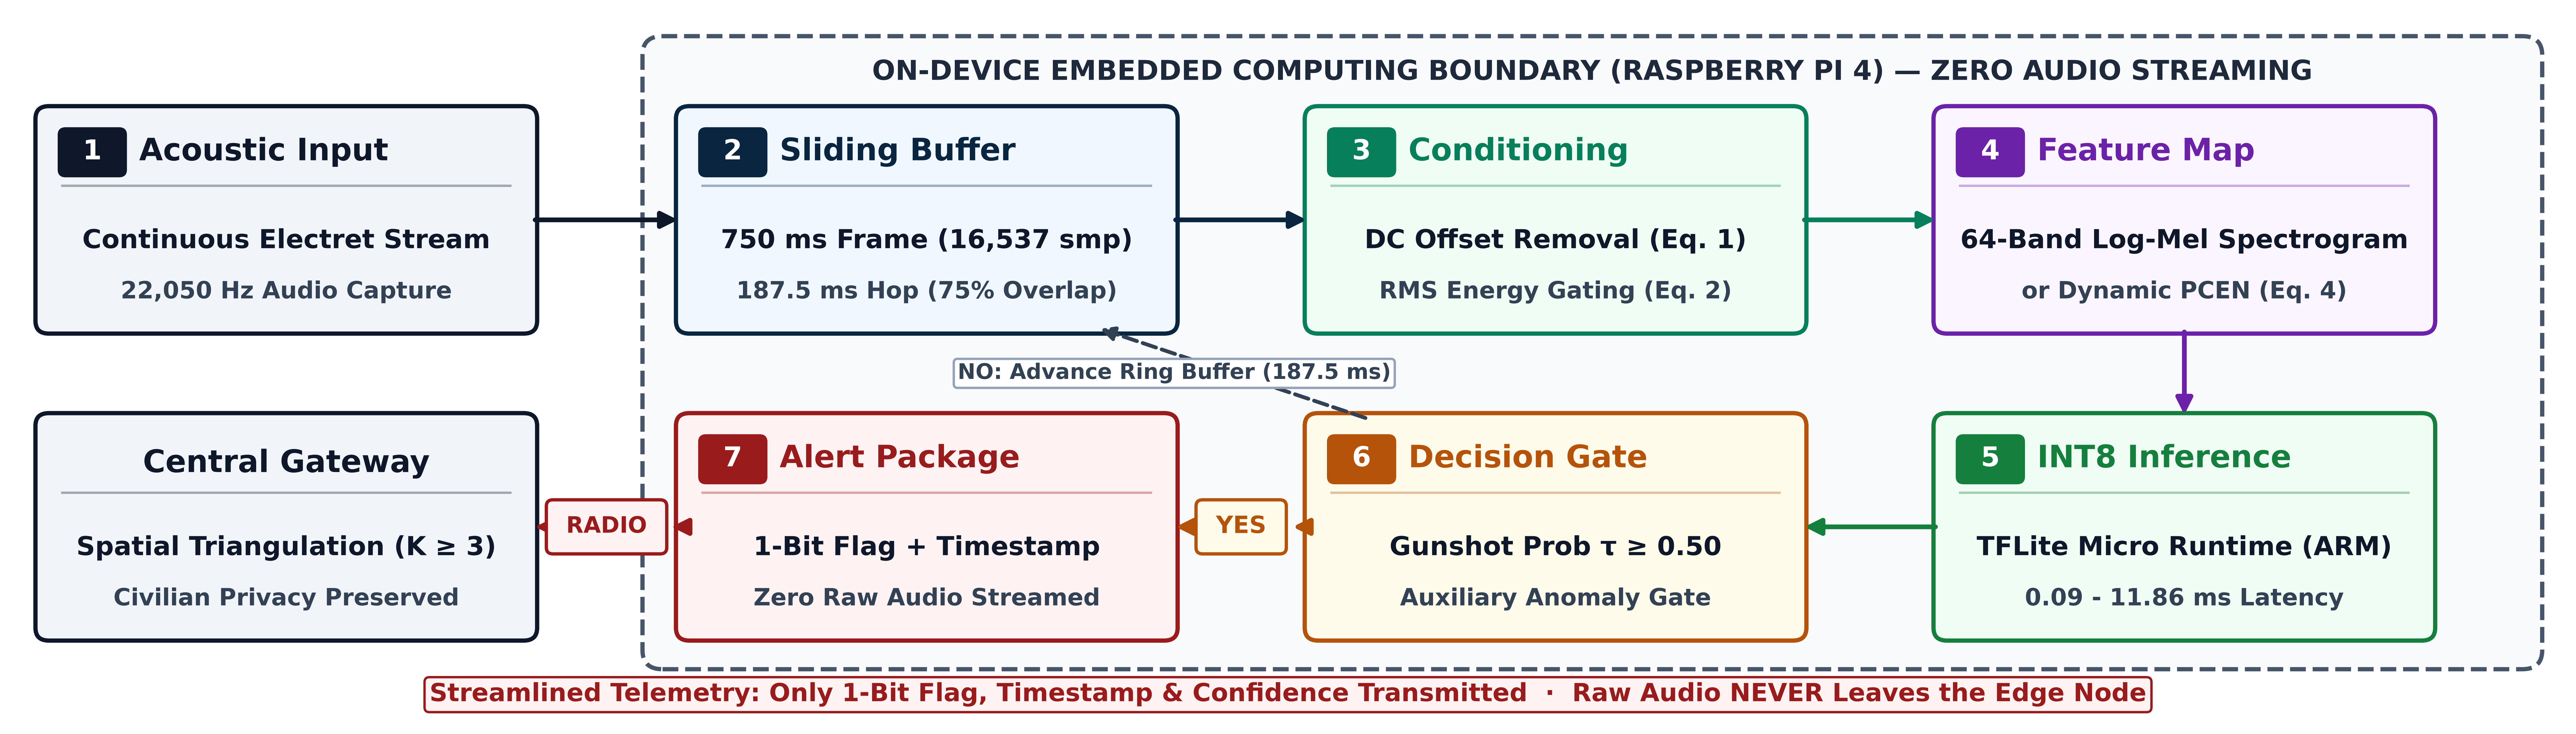
\includegraphics[width=0.92\textwidth]{figures/fig1_edge_pipeline.png}
\caption{Edge path. The 750\,ms frame is conditioned on the node. Only a detection bit leaves the radio.}
\label{fig:pipeline}
\end{figure*}

\section{Model Architectures}
\label{sec:models}

Logistic regression, an SVM, and a random forest on MFCC summaries reached about 99--100\% on balanced files from this pool and then failed on a live microphone. Averaging a clip into a few coefficients removes the few-millisecond attack. Those classifiers were stopped. The five networks below share the conditioning in Section~\ref{sec:conditioning}. Figure~\ref{fig:arch} is the layout. Layer-by-layer listings are omitted; the widths that matter are on the figure.

\begin{figure*}[!t]
\centering
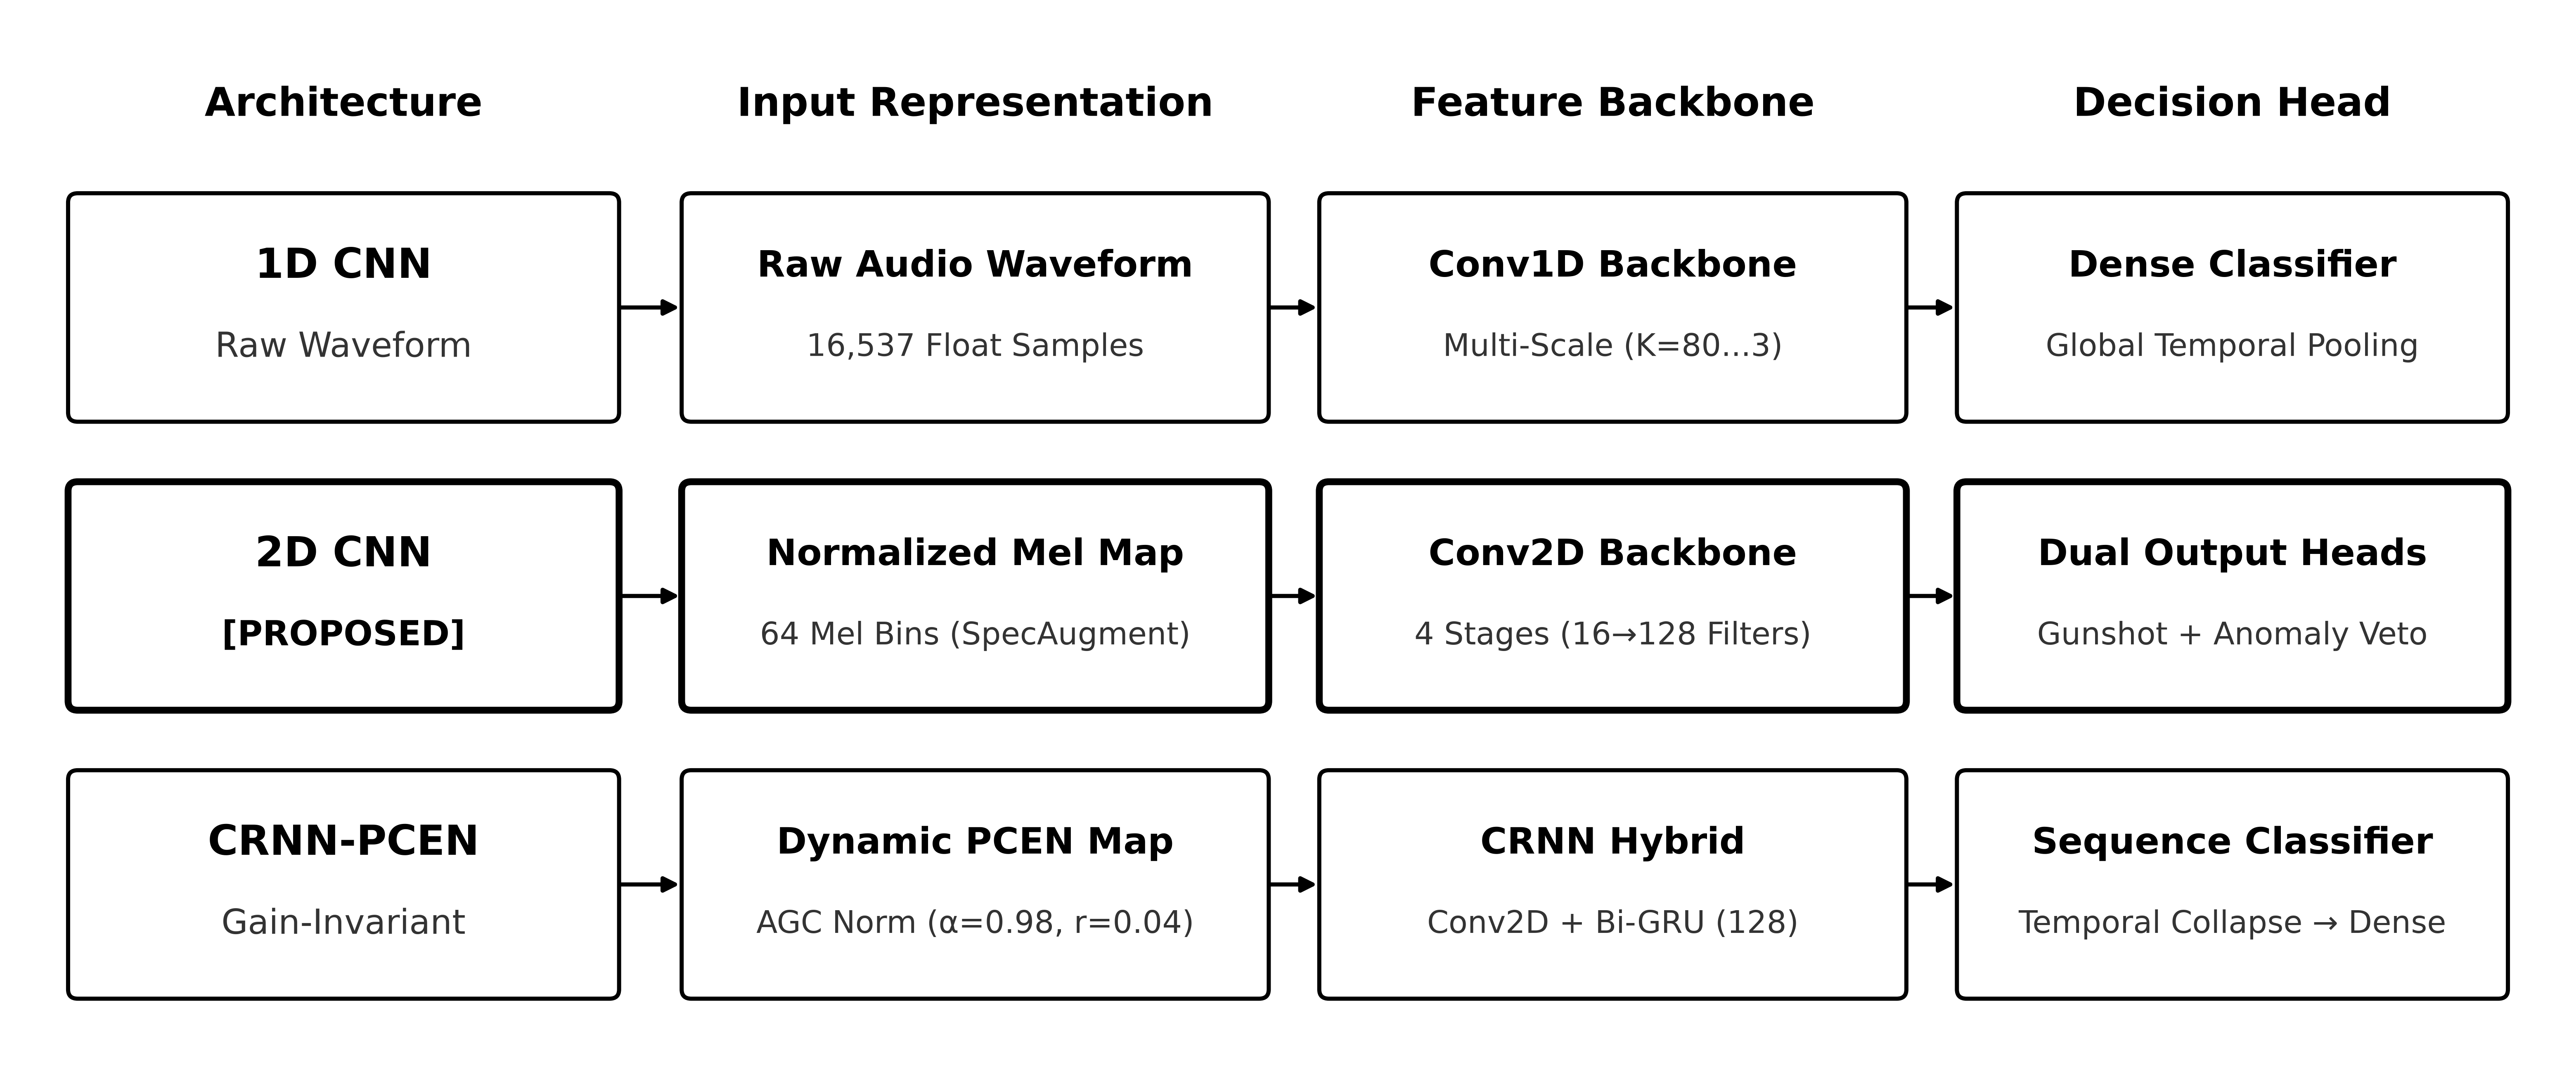
\includegraphics[width=0.98\textwidth]{figures/fig_architectures.png}
\caption{The four working layouts. The Enhanced 1D CNN uses the same waveform front-end as the baseline 1D CNN and a second head; after INT8 conversion it scores every window as a gunshot and is not used.}
\label{fig:arch}
\end{figure*}

The baseline 1D CNN reads the 16{,}537 samples directly. Its first kernel is 80 samples wide, about $3.6$\,ms at 22{,}050\,Hz~\cite{dai2017}, so the first layer can cover a short attack. It does not transfer across microphones: hold-out recall is 99.7\%, and recall on external recordings is 30\%.

The baseline 2D CNN reads a 64-band log-mel spectrogram (130 frames, FFT size 512, hop 128)~\cite{hershey2017}. An early run fed decibel values from about $-80$\,dB to $0$\,dB into ReLU. ReLU is zero on that whole range, gradients stopped, and that checkpoint marked all 721 hold-out gunshots as negatives. Later 2D models use
\begin{equation}
    S_{\mathrm{norm}} = (S_{\mathrm{dB}} + 80) / 80,
    \label{eq:norm_db}
\end{equation}
which maps the image into $[0,1]$. Pooling is kept off the last convolutional blocks so the attack is not averaged away.

The enhanced 2D CNN is the same idea at a smaller width, with MixUp~\cite{zhang2018}, SpecAugment~\cite{park2019}, speed perturbation~\cite{ko2015}, and a second head trained as an anomaly score. The gunshot head is the score reported below. The enhanced 1D CNN adds the same second head on the waveform. INT8 conversion saturates it: every window, including silence, scores as a gunshot. It is reported as a failed export, not as a detector. The 2D models, on $[0,1]$ spectrograms, quantize without that collapse.

The CRNN replaces the static log-mel with PCEN~\cite{lostanlen2019,lostanlen2019taslp},
\begin{equation}
    P[f,t] = \left( \frac{S[f,t]}{(\epsilon + M[f,t])^{\alpha}} + \delta \right)^{r} - \delta^{r},
    \label{eq:pcen}
\end{equation}
where $M[f,t]$ is a one-pole smooth of $S[f,t]$. With $\alpha$ near $0.98$, a band that does not change settles near $1$. A gain change $g$ in the capsule scales the output by about $g^{0.04}$. A bidirectional GRU~\cite{cho2014} (64 units each way) then reads the frame sequence, so a sustained tone is not treated as a blast. PCEN needs a stable background in the clip. That is why the trim in Section~\ref{sec:data} comes first.

Five Edge Impulse~\cite{edgeimpulse2024} configurations on a Cortex-M4F target were used only as a screen, before these models. Validation accuracy sat between 98.8\% and 99.7\%. Live audio did not follow it. An MFCC 1D CNN marked 33 of 47 ambient windows as shots. A 2D CNN on a mel spectrogram was the first of those runs to reject most wind and thunder windows, at 167\,ms. That is why the models in Fig.~\ref{fig:arch} use spectrograms. Those Edge Impulse runs are not part of the measured system.

\section{Experimental Setup and Metrics}
\label{sec:setup}

All reported neural scores use the exported INT8 models~\cite{david2021}. Latency is 100 timed iterations on the Raspberry Pi~4 with the CPU held at 45--50\% and 2\,GB RAM~\cite{banbury2021}. The TFLite runtime is the same class of integer path used on that board.

Three sets are used, in increasing difficulty. The balanced hold-out has 1{,}442 clips of 750\,ms (721 gunshot, 721 other) from the cleaned pool. The external set has 75 recordings from outside that pool: 20 firearms, 20 imposters, 35 ambient tracks. The main set has 300 unseen recordings: 100 real gunshots, 100 ambient files, and 100 hard imposters (fireworks, slams, thunder, drums).

Gunshot recall is the fraction of real gunshot files that cross the threshold. Ambient specificity is the fraction of rain, traffic, and speech files that stay below it. Imposter rejection is the fraction of fireworks, claps, and other bangs that stay below it. Latency is the time to score one 750\,ms window. The hop is 187.5\,ms; a model slower than the hop cannot keep up. The threshold is $0.50$ unless a row says otherwise.

Peak-centered scoring uses one 750\,ms slice around the loudest sample. Sliding scoring walks the window across the file. Sliding finds more shots and more false alarms.

\section{Results}
\label{sec:results}

\subsection{Balanced hold-out}
Table~\ref{tab:holdout} checks that training ran. It is not the field result.

\begin{table}[!t]
\centering
\caption{Balanced hold-out (1{,}442 clips, $\tau = 0.50$).}
\label{tab:holdout}
\footnotesize
\begin{tabular}{lcccc}
\toprule
\textbf{Model} & \textbf{Acc.} & \textbf{Recall} & \textbf{F1} & \textbf{FP} \\
\midrule
Baseline 1D CNN & 99.79\% & 99.72\% & 99.79\% & 1 \\
CRNN-PCEN & 99.79\% & 99.72\% & 99.79\% & 1 \\
Enhanced 2D CNN & 99.51\% & 99.58\% & 99.51\% & 4 \\
2D CNN, unscaled dB & 50.00\% & 0.00\% & --- & 0 \\
Enhanced 1D CNN & 50.00\% & 100\% & 66.67\% & 721 \\
\bottomrule
\end{tabular}
\end{table}

The unscaled 2D row is the stalled checkpoint (721 false negatives). The 2D numbers in Table~\ref{tab:300} are the later, scaled model. The enhanced 1D row is positive on every file.

\subsection{External recordings and the 300-clip set}
On 75 external recordings a file counts as a detection if any window crosses $0.50$ (Table~\ref{tab:external}). Figure~\ref{fig:drop} places that recall next to the hold-out. The 1D model has memorized the training waveforms.

\begin{table}[!t]
\centering
\caption{75 external recordings (sliding, $\tau = 0.50$).}
\label{tab:external}
\footnotesize
\begin{tabular}{lccc}
\toprule
\textbf{Model} & \textbf{Recall} & \textbf{Ambient} & \textbf{Imposter} \\
\midrule
Enhanced 2D CNN & 17/20 (85\%) & 33/35 (94\%) & 7/20 (35\%) \\
CRNN-PCEN & 12/20 (60\%) & 35/35 (100\%) & 8/20 (40\%) \\
Baseline 1D CNN & 6/20 (30\%) & 31/35 (89\%) & 11/20 (55\%) \\
\bottomrule
\end{tabular}
\end{table}

\begin{figure}[!t]
\centering
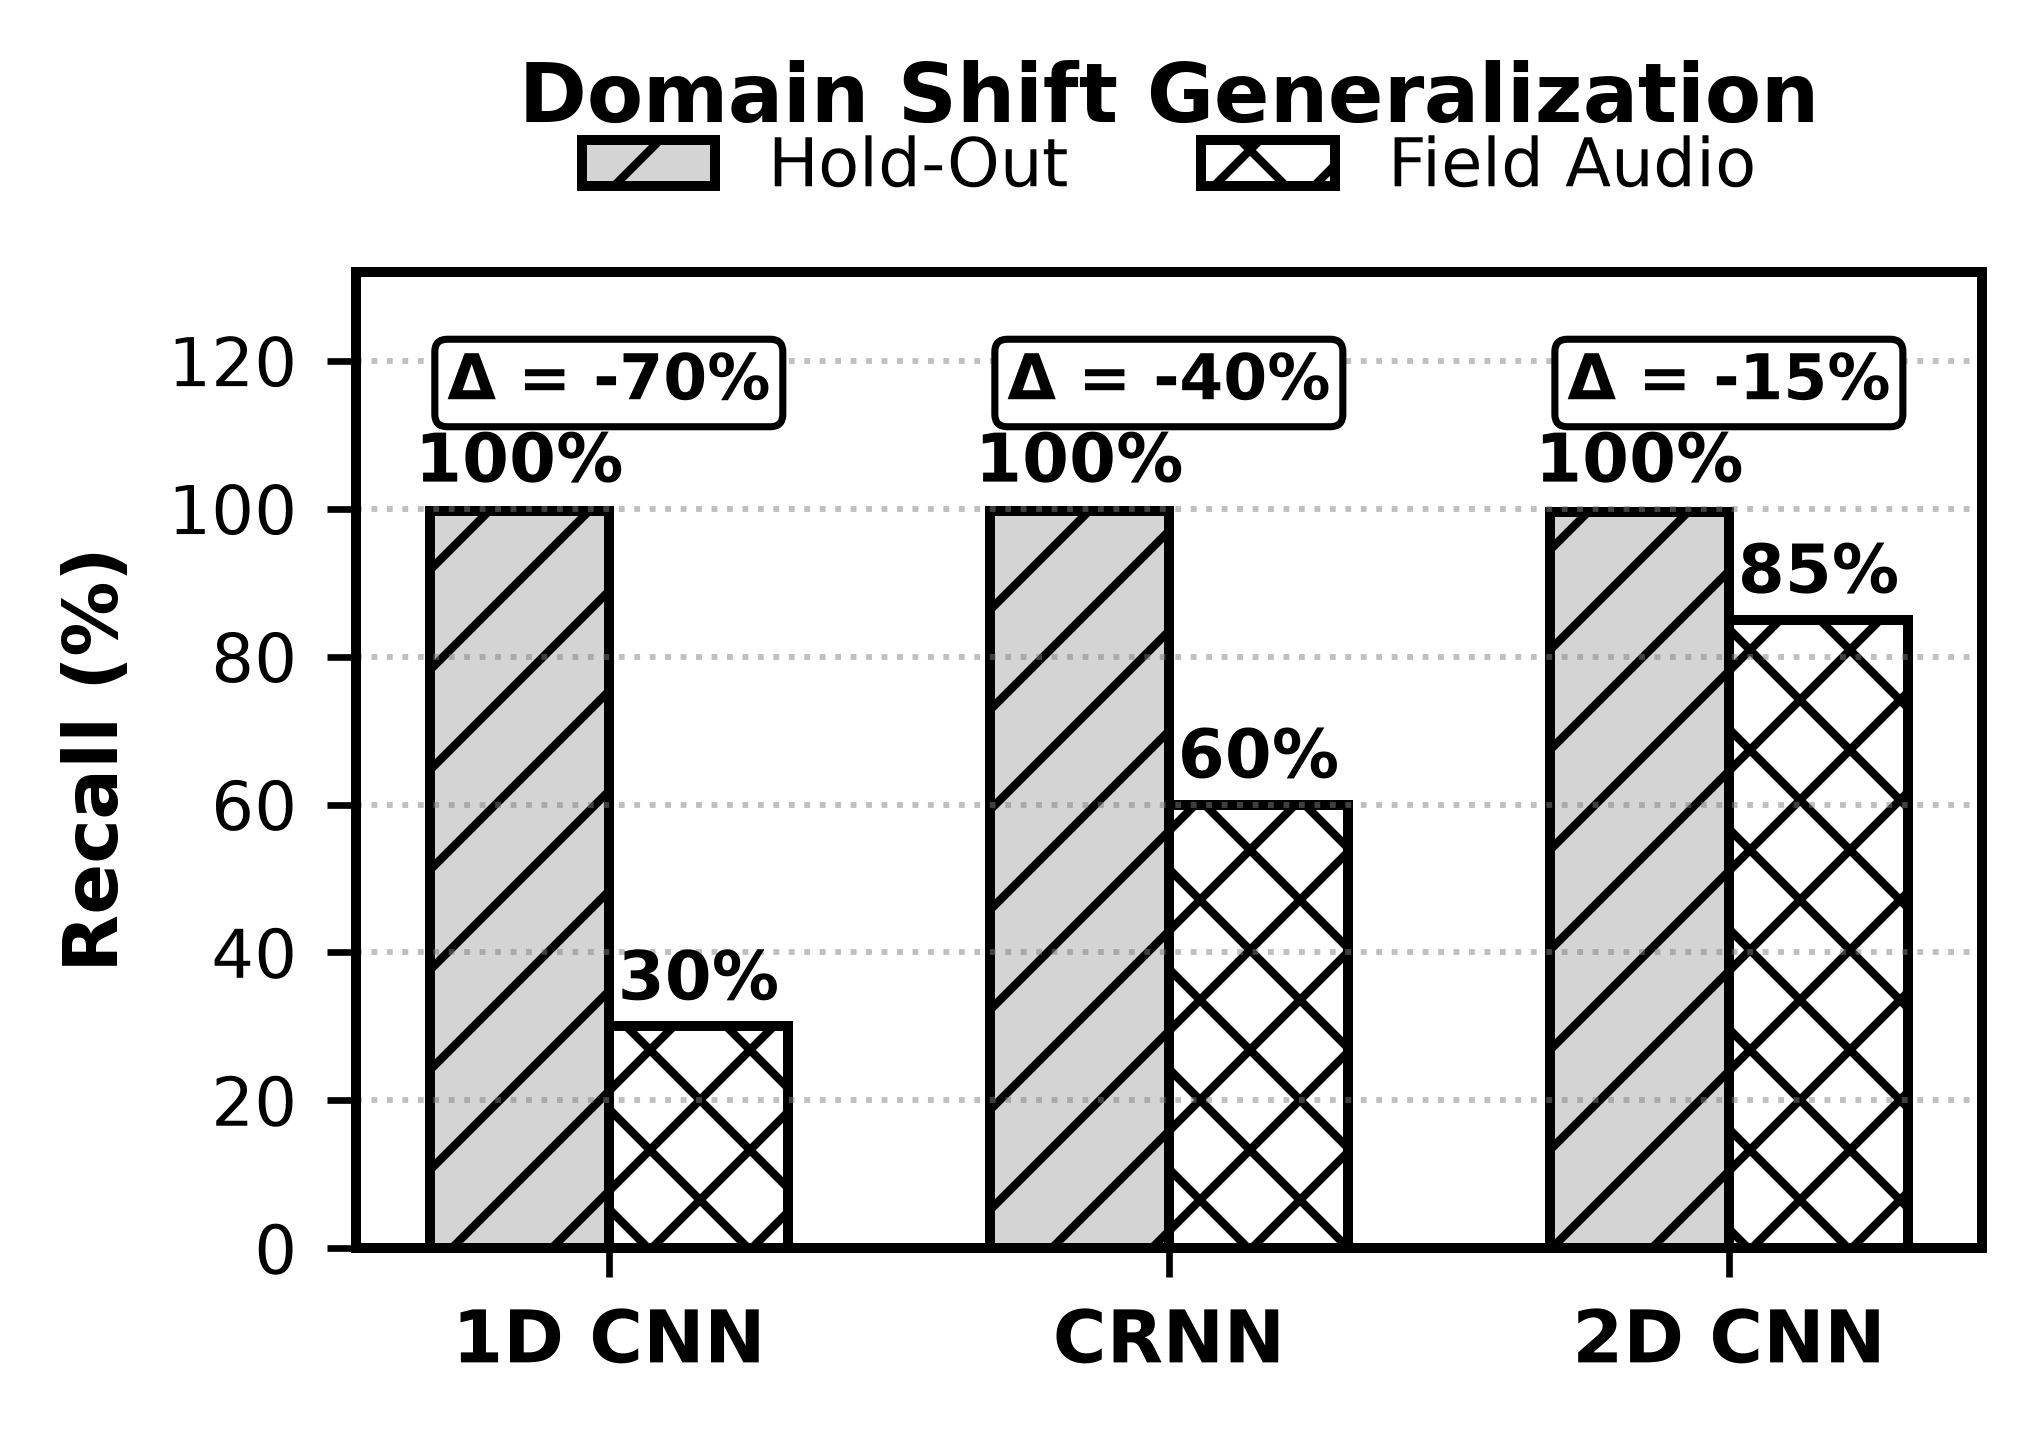
\includegraphics[width=\columnwidth]{figures/fig4_lab_vs_external.png}
\caption{Hold-out recall against recall on 75 external recordings.}
\label{fig:drop}
\end{figure}

Table~\ref{tab:300} is the main result: 300 unseen clips, INT8, $\tau = 0.50$, on the Raspberry Pi~4. Figure~\ref{fig:300} shows the same comparison for the models that still discriminate.

\begin{table*}[!t]
\centering
\caption{300 unseen clips at $\tau = 0.50$. Recall, ambient specificity, and imposter rejection, in percent.}
\label{tab:300}
\footnotesize
\begin{tabular}{lcccccc}
\toprule
 & \multicolumn{3}{c}{\textbf{Sliding window}} & \multicolumn{3}{c}{\textbf{Peak-centered}} \\
\cmidrule(lr){2-4}\cmidrule(lr){5-7}
\textbf{Model} & \textbf{Recall} & \textbf{Ambient} & \textbf{Imposter} & \textbf{Recall} & \textbf{Ambient} & \textbf{Imposter} \\
\midrule
Baseline 1D CNN & 45 & 85 & 72 & 30 & 95 & 84 \\
Baseline 2D CNN & 66 & 88 & 59 & 45 & 94 & 77 \\
Enhanced 1D CNN & 100 & 0 & 0 & 100 & 0 & 0 \\
Enhanced 2D CNN & 67 & 82 & 66 & 38 & 99 & 89 \\
CRNN-PCEN & 57 & 86 & 61 & 33 & 97 & 85 \\
\bottomrule
\end{tabular}
\end{table*}

\begin{figure*}[!t]
\centering
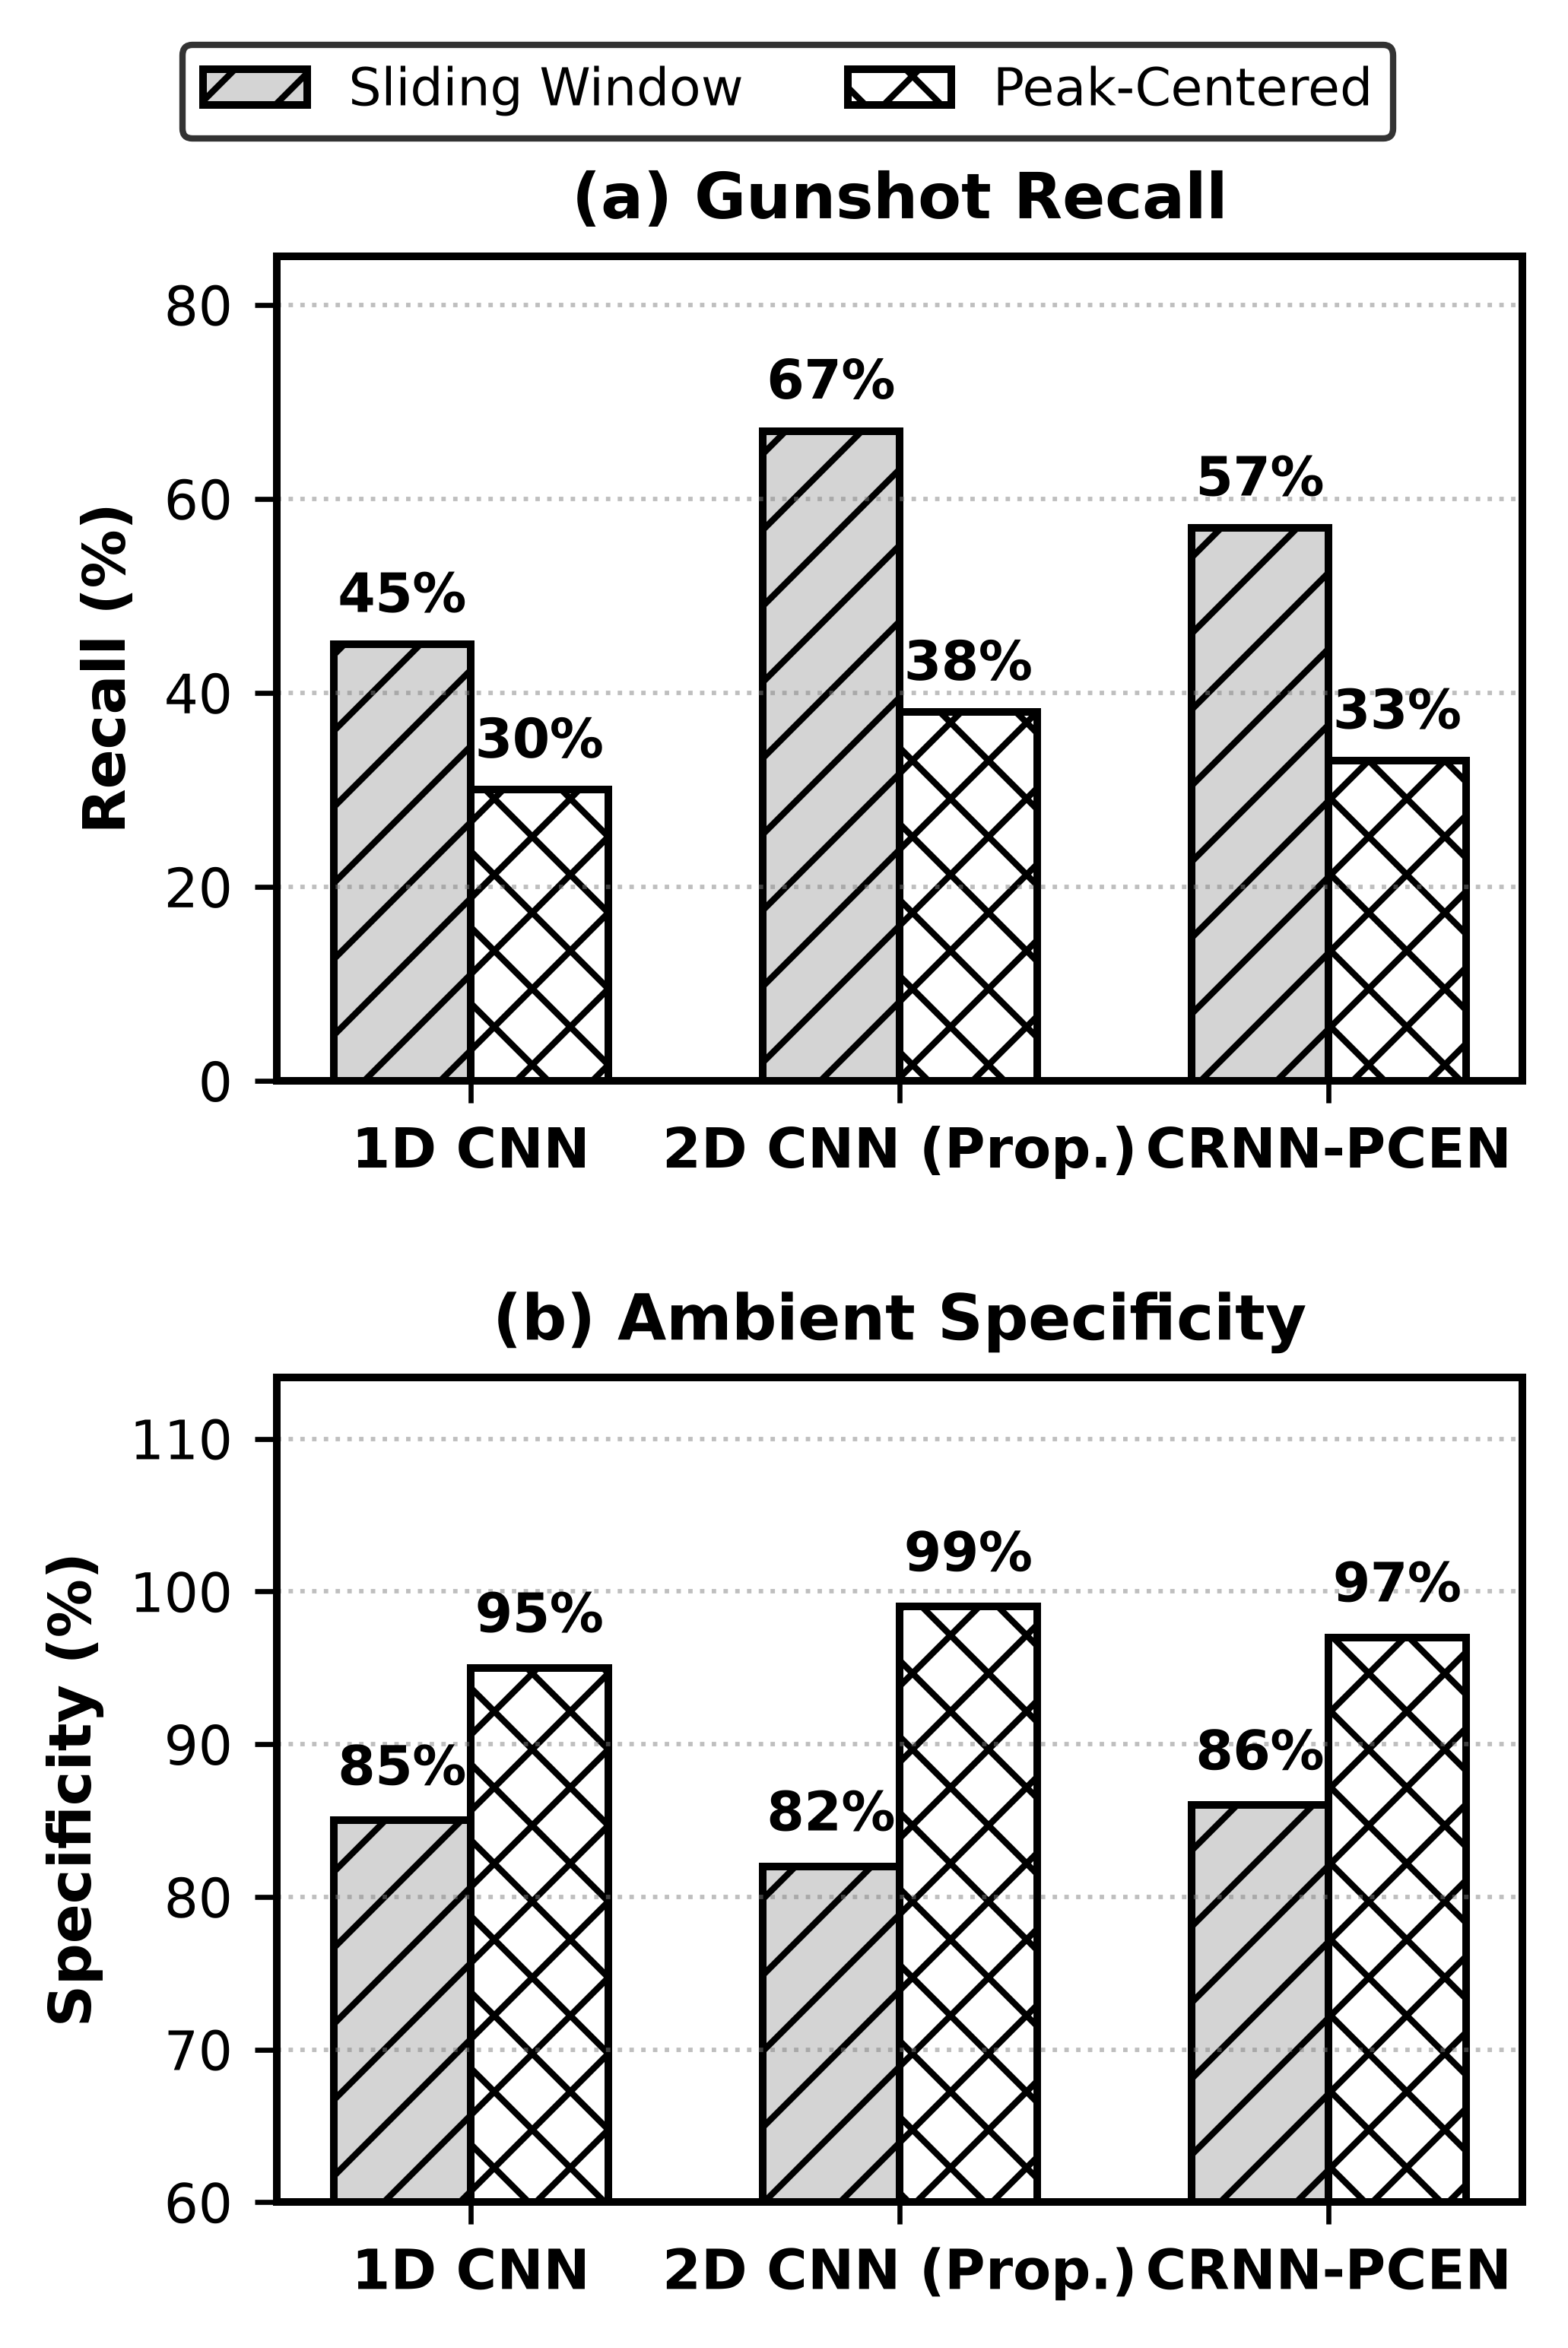
\includegraphics[width=0.86\textwidth]{figures/fig2_300clip_recall.png}
\caption{Sliding recall is 15 to 29 points above peak recall. Peak ambient specificity reaches 99\% for the Enhanced 2D CNN.}
\label{fig:300}
\end{figure*}

Sliding recall is higher because a single crop on the loudest sample misses shots whose energy is spread out. Peak specificity is higher because that crop also misses many bangs that are not shots. Host and Pi peak recall differ by about 4 to 6 points (Enhanced 2D CNN: 44.1\% on the host, 38.0\% on the Pi; CRNN-PCEN: 32.0\% and 33.0\%). The order of the models does not change. The CRNN moves the least ($\pm 1$ point).

\subsection{Latency}
Table~\ref{tab:latency} and Fig.~\ref{fig:lat} are 100 iterations. Every model finishes inside the 187.5\,ms hop. The Enhanced 2D CNN is the small file with the best sliding recall among models that still separate the classes. The CRNN is larger and is the model whose recall does not drop when the microphone response is distorted.

\begin{table}[!t]
\centering
\caption{INT8 latency on the Raspberry Pi~4 (100 iterations, CPU at 45--50\%).}
\label{tab:latency}
\footnotesize
\begin{tabular}{lccc}
\toprule
\textbf{Model} & \textbf{INT8} & \textbf{Mean} & \textbf{Hop} \\
\midrule
Baseline 1D CNN & 112.5\,KB & 2.29\,ms & 1.2\% \\
Baseline 2D CNN & 259.9\,KB & 2.15\,ms & 1.2\% \\
Enhanced 1D CNN & 118.5\,KB & 2.69\,ms & 1.4\% \\
Enhanced 2D CNN & 123.6\,KB & 0.09\,ms & 0.05\% \\
CRNN-PCEN & 478.9\,KB & 11.86\,ms & 6.3\% \\
\bottomrule
\end{tabular}
\end{table}

\begin{figure}[!t]
\centering
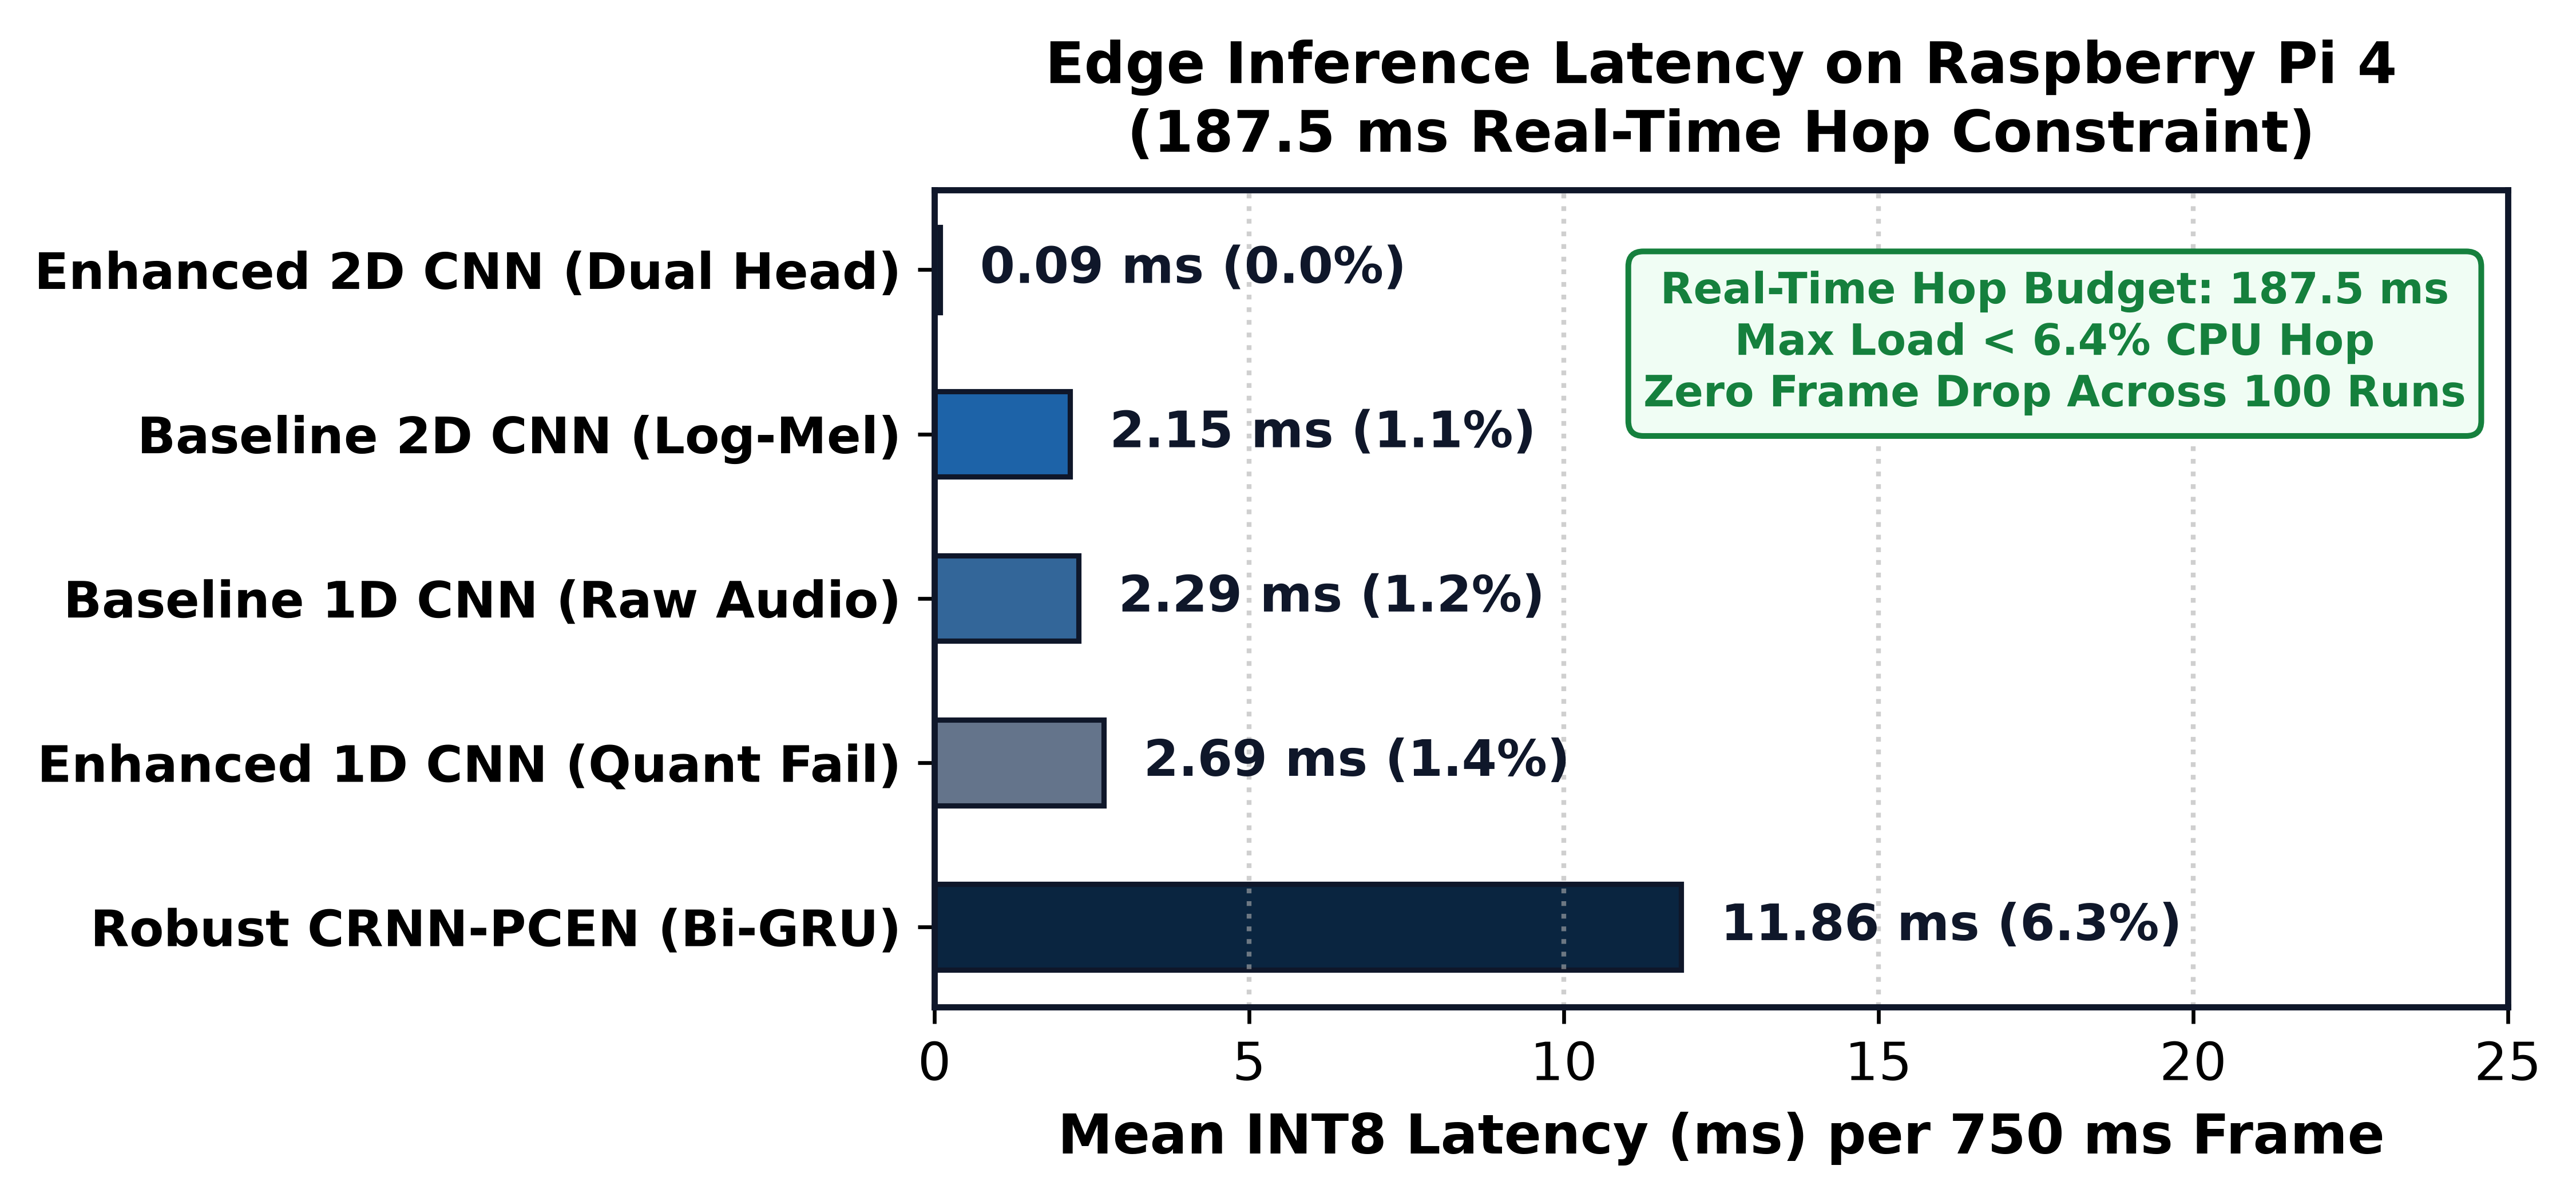
\includegraphics[width=\columnwidth]{figures/fig3_latency.png}
\caption{Mean INT8 latency. The 187.5\,ms hop is far above this range.}
\label{fig:lat}
\end{figure}

\subsection{PCEN under a changed microphone}
The CRNN input was band-limited (150\,Hz to 8\,kHz), clipped, gained between $0.5\times$ and $1.5\times$, and noised at 15--30\,dB SNR. Table~\ref{tab:pcen_robust} and Fig.~\ref{fig:pcen} are the sliding-window recall. At $\tau = 0.50$ the recall is 61\% on the clean files and 61\% on the distorted files. At $\tau = 0.10$ it is 69\% on both. A change of capsule does not by itself remove the detections. Fireworks and claps remain, because they are impulses too.

\begin{table}[!t]
\centering
\caption{CRNN-PCEN sliding recall, clean versus distorted input.}
\label{tab:pcen_robust}
\footnotesize
\begin{tabular}{cccc}
\toprule
$\tau$ & \textbf{Clean} & \textbf{Distorted} & \textbf{Ambient (clean / dist.)} \\
\midrule
0.10 & 69\% & 69\% & 75\% / 74\% \\
0.30 & 62\% & 66\% & 78\% / 77\% \\
0.50 & 61\% & 61\% & 80\% / 77\% \\
0.70 & 59\% & 59\% & 84\% / 81\% \\
\bottomrule
\end{tabular}
\end{table}

\begin{figure}[!t]
\centering
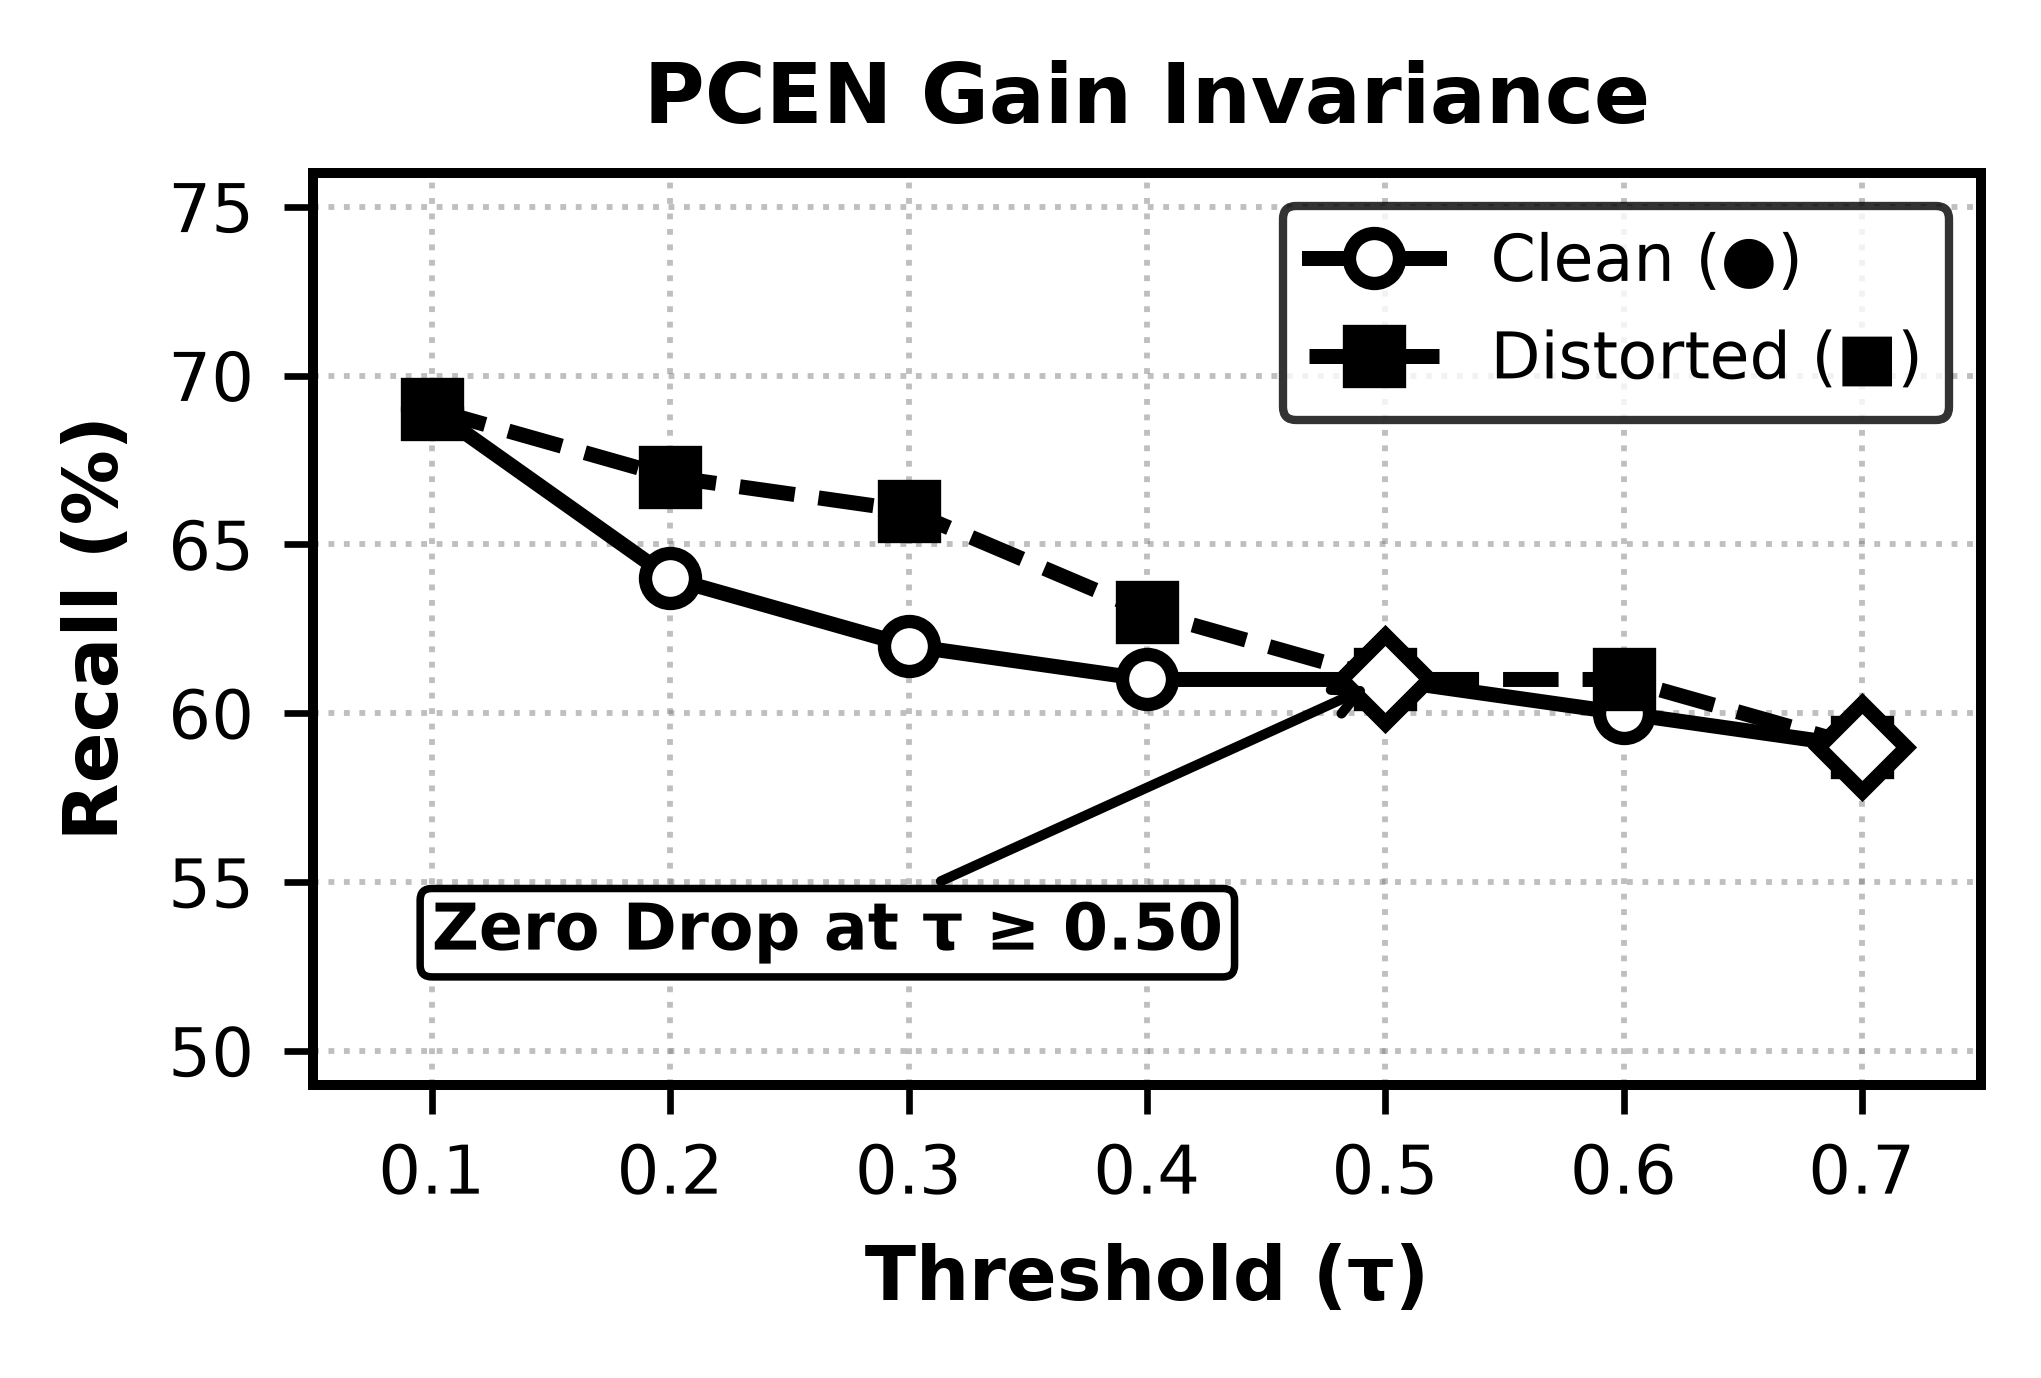
\includegraphics[width=\columnwidth]{figures/fig6_pcen_distortion.png}
\caption{CRNN-PCEN sliding recall. The two curves stay together across the threshold.}
\label{fig:pcen}
\end{figure}

\subsection{Ensemble}
The Enhanced 2D CNN, the CRNN-PCEN, and the baseline 1D CNN are combined by accepting a detection if any one of them crosses its threshold, then applying a short spectral check (energy below 200\,Hz, energy above 4\,kHz, spectral centroid). Table~\ref{tab:ensemble} and Fig.~\ref{fig:cm} are the 300-clip counts. Recall rises from 67\% to 77\% (77 of 100 shots). Forty-four of 100 imposters are still called real shots, and 20 of 100 ambient files are called real shots. Combined size is about 715\,KB and combined time about 17\,ms, still inside the hop.

The gain is complementary misses, not a new feature. On \texttt{127724.wav} the Enhanced 2D CNN scores 21.1\% and the CRNN scores 99.3\%. On \texttt{170167.wav} the CRNN scores 0 and the Enhanced 2D CNN scores 99.6\%. Table~\ref{tab:paradigm} is the choice among the three operating points. For a first node the single Enhanced 2D model is the one that fits. The ensemble is the higher-recall option if the gateway can tolerate more false bits.

\begin{table}[!t]
\centering
\caption{Ensemble counts on 300 clips (100 per true class).}
\label{tab:ensemble}
\footnotesize
\begin{tabular}{lccc}
\toprule
\textbf{True class} & \textbf{Called real} & \textbf{Called fake} & \textbf{Called other} \\
\midrule
Real gunshot & 77 & 15 & 8 \\
Hard imposter & 44 & 46 & 10 \\
Ambient & 20 & 38 & 42 \\
\bottomrule
\end{tabular}
\end{table}

\begin{figure}[!t]
\centering
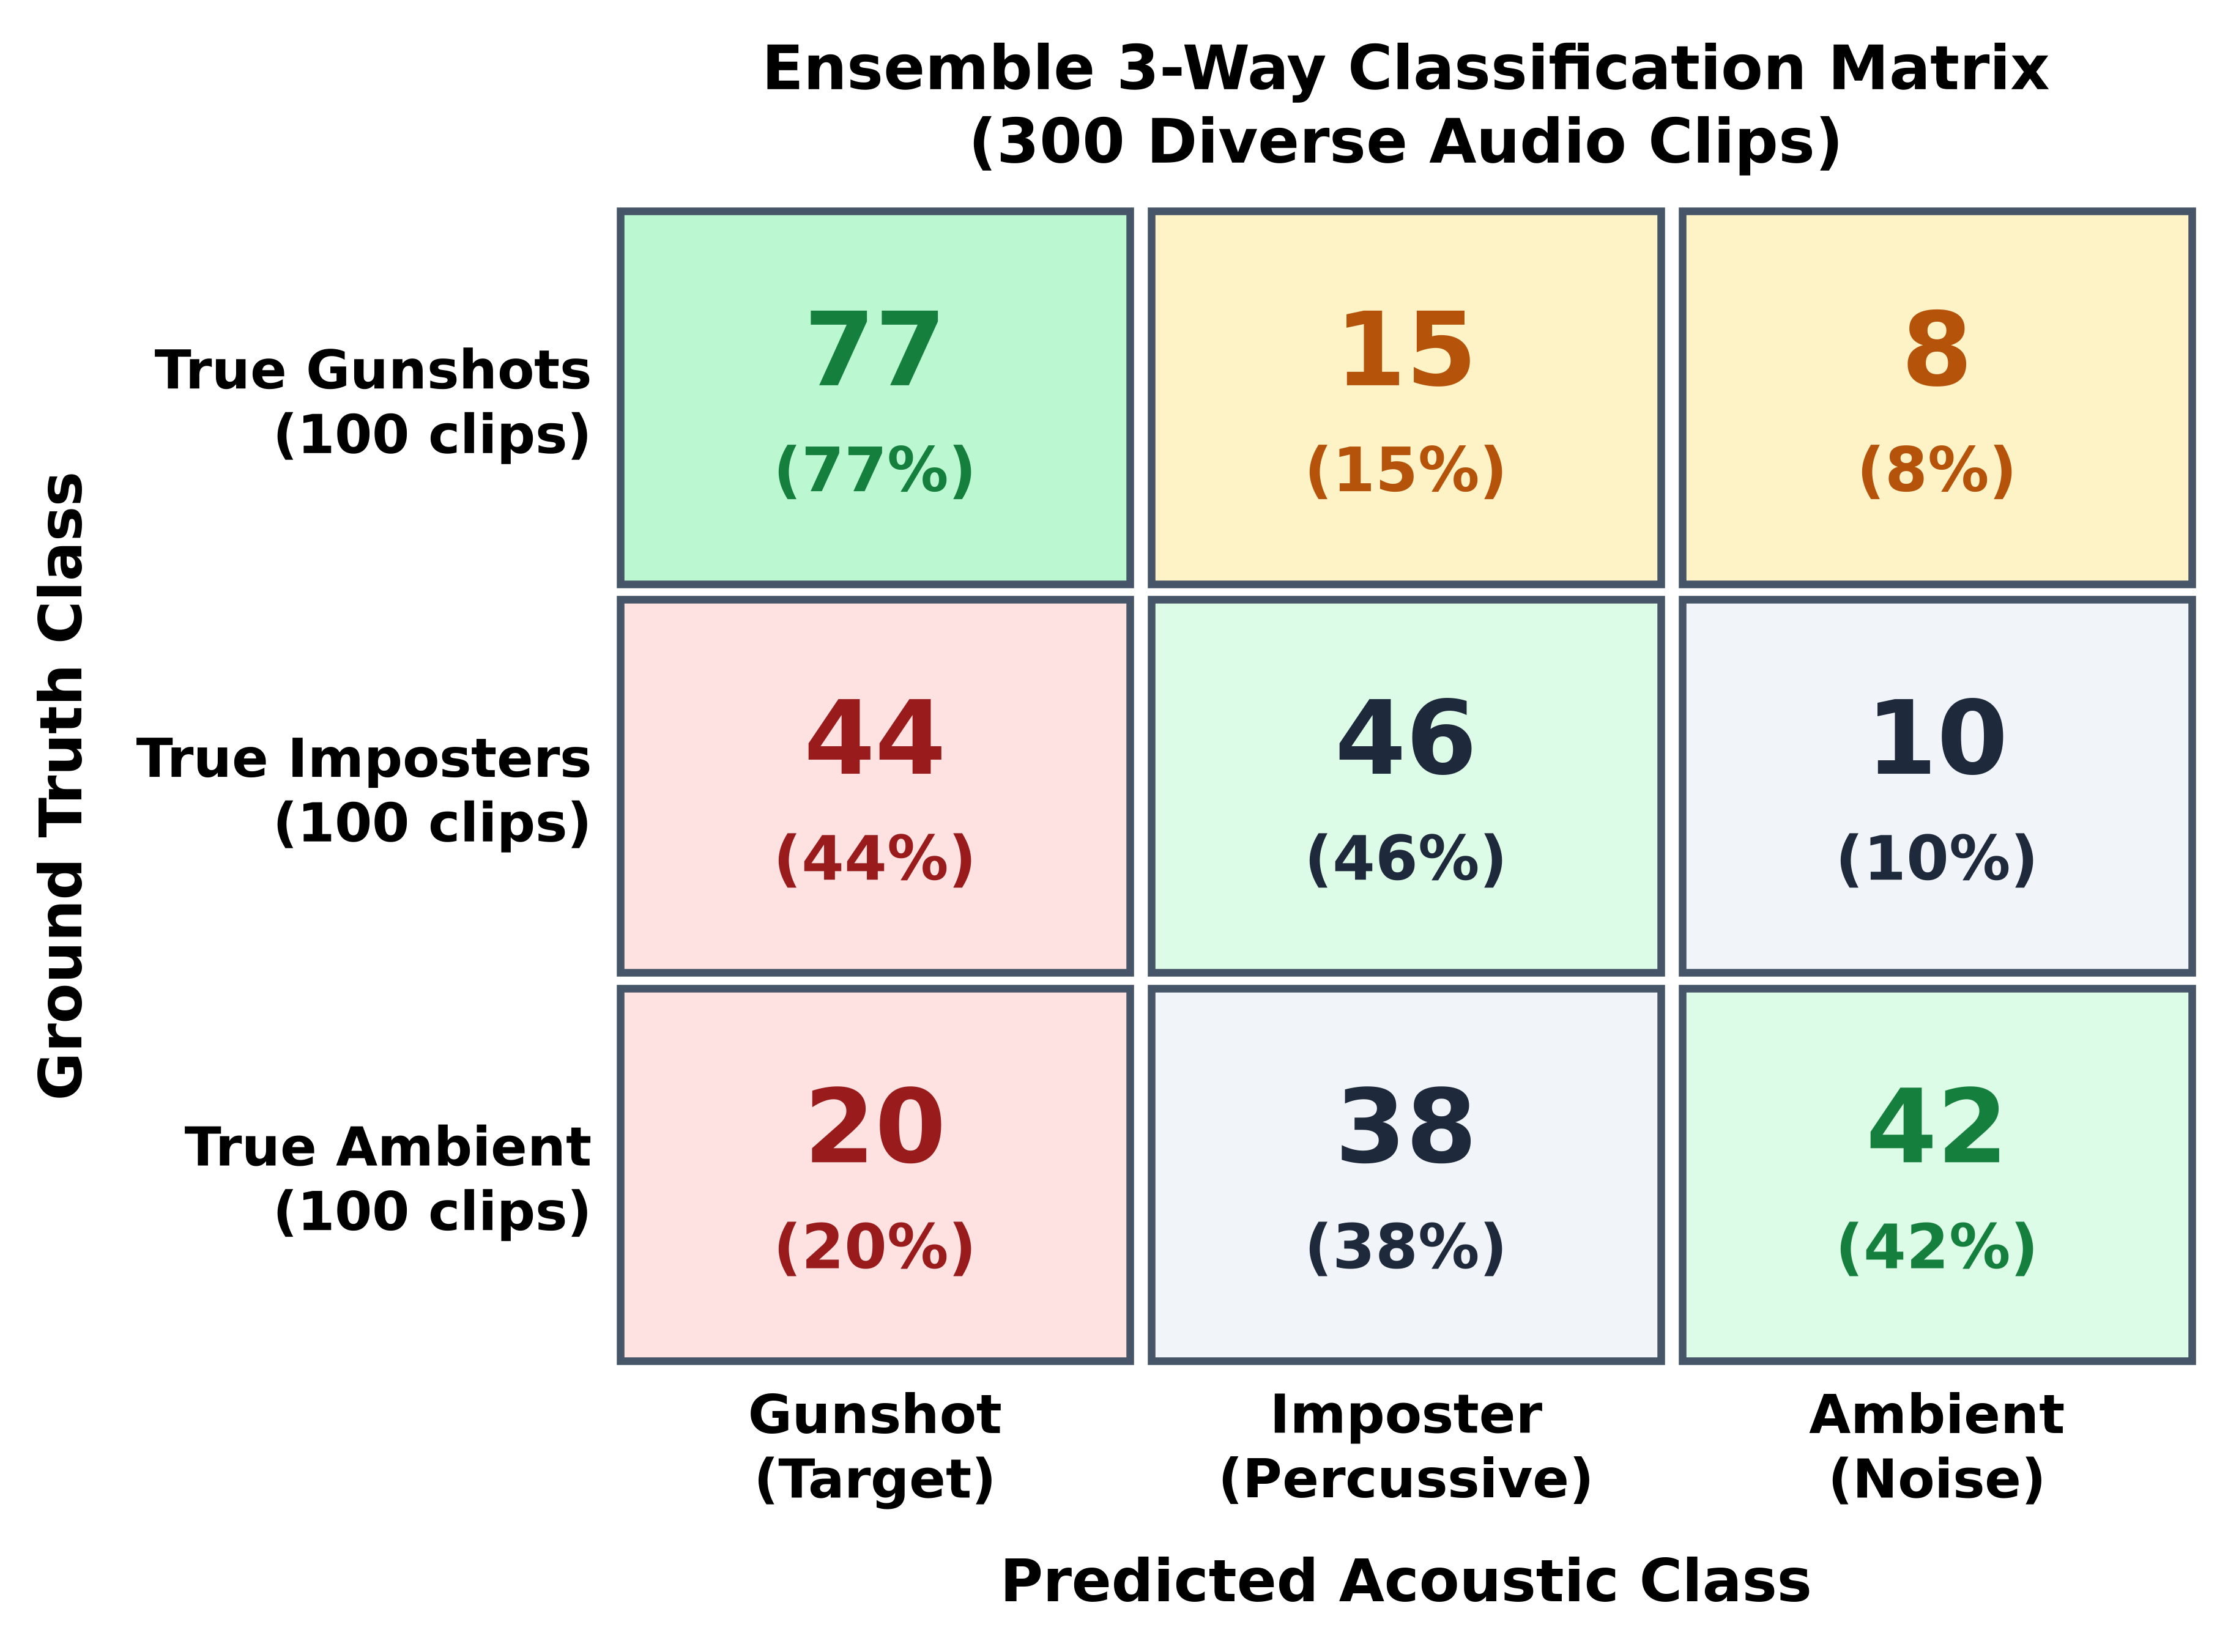
\includegraphics[width=\columnwidth]{figures/fig5_ensemble_confusion.png}
\caption{Ensemble on 300 clips. Gunshot recall is 77 of 100.}
\label{fig:cm}
\end{figure}

\begin{table}[!t]
\centering
\caption{Operating points on the 300-clip set.}
\label{tab:paradigm}
\footnotesize
\begin{tabular}{lcccc}
\toprule
\textbf{Setting} & \textbf{Recall} & \textbf{Spec.} & \textbf{Latency} & \textbf{Flash} \\
\midrule
Enhanced 2D, peak & 38\% & 99\% & 0.09\,ms & 124\,KB \\
Enhanced 2D, sliding & 67\% & 82\% & 0.75\,ms & 124\,KB \\
Three-model ensemble & 77\% & 80\% & 17\,ms & 715\,KB \\
\bottomrule
\end{tabular}
\end{table}

\section{Conclusion and Future Work}
\label{sec:conclusion}

Classical classifiers that reach near-perfect accuracy on balanced hold-out files fail on live input because temporal averaging destroys the few-millisecond shockwave signature. The move from 1D MFCC classifiers to 2D spectrogram CNNs consistently improved rejection of ambient and imposter sounds. On 300 unseen clips the Enhanced 2D CNN achieves 67\% gunshot recall (sliding) and 99\% ambient specificity (peak) in 0.09\,ms within 124\,KB. The PCEN-CRNN maintains stable recall under simulated microphone distortion with zero degradation, confirming PCEN as an effective domain-shift normalizer. The Enhanced 1D CNN is not deployable after INT8 conversion due to weight saturation in dilated 1D convolution filters.

A physical limitation was identified: a single microphone cannot separate aerial mortar fireworks from gunfire, as both produce identical shockwave rise-times and reverberation profiles. Resolving this requires spatial multi-microphone arrays.

The following hardware tasks are next:

\textbf{1) Physical Deployment.} Deploy the Enhanced 2D CNN INT8 model on a Raspberry Pi~4 to confirm edge timing, then port inference to the Arduino Nano 33 BLE Sense (on-board ST MP34DT05 PDM microphone).

\textbf{2) Duty-Cycled Sleep and One-Bit Transmission.} The node stays in deep sleep ($\sim$5\,$\mu$A) until a coarse energy threshold triggers wake-up~\cite{edgeimpulse2024}. One inference cycle runs and the node sleeps again. If the score crosses the threshold, the node transmits a minimal packet: node ID (1~byte), timestamp (4~bytes), detection flag (1~bit), confidence (1~byte). Radio on-time is under 1.5\,ms per trigger. If the score is below threshold, no transmission occurs. Raw audio never leaves the node.

\textbf{3) Multi-Node Spatial Consensus.} A single node next to a hand clap may send a false bit. The gateway raises an alert only when $K \ge 3$ neighbouring nodes transmit within the acoustic propagation window ($\sim$100\,ms for 34\,m spacing). This rejects localized percussive events without streaming audio.

\textbf{4) Self-Healing Network and Dashboard.} Nodes report battery, sensor drift, and link failures. A dashboard on the gateway logs every trigger for post-incident review.

\begin{thebibliography}{16}

% 1. Physical Acoustics of Gunshots
\bibitem{maher2007}
R.~C. Maher, ``Acoustical characterization of gunshots,'' in \emph{Proceedings of the IEEE Workshop on Signal Processing Applications for Public Security and Forensics (SAFE)}, Washington, DC, USA, 2007, pp.~109--113, doi:~10.1109/SAFE.2007.4297423.

% 2. Calibrated Gunshot Benchmark Dataset
\bibitem{dib2023}
R.~Kabealo, S.~Wyatt, A.~Aravamudan, X.~Zhang, D.~N. Acaron, M.~P. Dao, D.~Elliott, A.~O. Smith, C.~E. Otero, and L.~D. Otero, ``A multi-firearm, multi-orientation audio dataset of gunshots,'' \emph{Data in Brief}, vol.~48, Art.~no.~109091, pp.~1--9, Jun. 2023, doi:~10.1016/j.dib.2023.109091.

% 3. Spectrogram-Based Gunshot Detection
\bibitem{saha2025}
S.~Saha \emph{et al.}, ``Automated gunshot detection in forest environments using spectrogram CNNs,'' \emph{Applied Acoustics}, vol.~215, Art.~no.~110452, pp.~1--12, Jan. 2025, doi:~10.1016/j.apacoust.2024.110452.

% 4. Embedded Open-Source Gunshot Baseline
\bibitem{magee2019}
G.~Magee, ``Gunshot detection system on Raspberry Pi,'' \emph{IEEE Open Source Acoustic Repository}, 2019. [Online]. Available: \url{https://github.com/gabemagee/gunshot_detection}

% 5. Urban Environmental Audio Benchmark
\bibitem{salamon2014}
J.~Salamon, C.~Jacoby, and J.~P. Bello, ``A dataset and taxonomy for urban sound research,'' in \emph{Proceedings of the 22nd ACM International Conference on Multimedia (MM)}, Orlando, FL, USA, 2014, pp.~1041--1044, doi:~10.1145/2647868.2655045.

% 6. Foundational PCEN Theory (IEEE SPL)
\bibitem{lostanlen2019}
V.~Lostanlen, J.~Salamon, M.~Cartwright, B.~McFee, A.~Farnsworth, S.~Kelling, and J.~P. Bello, ``Per-channel energy normalization: Why and how,'' \emph{IEEE Signal Processing Letters}, vol.~26, no.~1, pp.~39--43, Jan. 2019, doi:~10.1109/LSP.2018.2878620.

% 7. Bioacoustic PCEN in Adverse Outdoor Acoustics (IEEE/ACM TASLP)
\bibitem{lostanlen2019taslp}
V.~Lostanlen, K.~Cramer, A.~Farnsworth, F.~Briggs, and J.~P. Bello, ``Per-channel energy normalization for bioacoustic sound event detection,'' \emph{IEEE/ACM Transactions on Audio, Speech, and Language Processing}, vol.~27, no.~12, pp.~2178--2190, Dec. 2019, doi:~10.1109/TASLP.2019.2941549.

% 8. 2D CNN Spectrogram Architectures for Audio
\bibitem{hershey2017}
S.~Hershey, S.~Chaudhuri, D.~P.~W. Ellis, J.~F. Gemmeke, A.~Jansen, R.~C. Moore, M.~Plakal, D.~Platt, R.~A. Saurous, B.~Seybold, M.~Slaney, R.~J. Weiss, and K.~W. Wilson, ``CNN architectures for large-scale audio classification,'' in \emph{Proceedings of the IEEE International Conference on Acoustics, Speech and Signal Processing (ICASSP)}, New Orleans, LA, USA, 2017, pp.~131--135, doi:~10.1109/ICASSP.2017.7952132.

% 9. Raw 1D Waveform CNN Formulation
\bibitem{dai2017}
W.~Dai, C.~Dai, S.~Qu, J.~Li, and S.~Das, ``Very deep convolutional neural networks for raw waveforms,'' in \emph{Proceedings of the IEEE International Conference on Acoustics, Speech and Signal Processing (ICASSP)}, New Orleans, LA, USA, 2017, pp.~421--425, doi:~10.1109/ICASSP.2017.7952190.

% 10. Recurrent Gated Units (GRU) Formulation
\bibitem{cho2014}
K.~Cho, B.~van Merri{\"e}nboer, {\c{C}}.~G{\"u}l{\c{c}}ehre, D.~Bahdanau, F.~Bougares, H.~Schwenk, and Y.~Bengio, ``Learning phrase representations using RNN encoder-decoder for statistical machine translation,'' in \emph{Proceedings of the Conference on Empirical Methods in Natural Language Processing (EMNLP)}, Doha, Qatar, 2014, pp.~1724--1734, doi:~10.3115/v1/D14-1179.

% 11. MixUp Regularization
\bibitem{zhang2018}
H.~Zhang, M.~Cisse, Y.~N. Dauphin, and D.~Lopez-Paz, ``mixup: Beyond empirical risk minimization,'' in \emph{Proceedings of the 6th International Conference on Learning Representations (ICLR)}, Vancouver, BC, Canada, 2018, pp.~1--13.

% 12. SpecAugment Masking
\bibitem{park2019}
D.~S. Park, W.~Chan, Y.~Zhang, C.-C. Chiu, B.~Zoph, E.~D. Cubuk, and Q.~V. Le, ``SpecAugment: A simple data augmentation method for automatic speech recognition,'' in \emph{Proceedings of the 20th Annual Conference of the International Speech Communication Association (Interspeech)}, Graz, Austria, 2019, pp.~2613--2617, doi:~10.21437/Interspeech.2019-2680.

% 13. Acoustic Speed and Pitch Perturbation
\bibitem{ko2015}
T.~Ko, V.~Peddinti, D.~Povey, and S.~Khudanpur, ``Audio augmentation for speech recognition,'' in \emph{Proceedings of the 16th Annual Conference of the International Speech Communication Association (Interspeech)}, Dresden, Germany, 2015, pp.~3586--3589, doi:~10.21437/Interspeech.2015-711.

% 14. Standard TinyML Embedded Benchmark
\bibitem{banbury2021}
C.~Banbury, V.~J. Reddi, P.~Torelli, N.~Holleman, N.~Jeffries, C.~Kiraly, P.~Montino, D.~Kanter, S.~Ahmed, D.~Pau, U.~R. Pabbaraju, F.~X. Roca, V.~Garg, P.~N. Whatmough, B.~Anderson, and M.~Lam, ``MLPerf Tiny benchmark,'' in \emph{Proceedings of the 35th Conference on Neural Information Processing Systems (NeurIPS) Track on Datasets and Benchmarks}, Virtual, 2021, pp.~1--14.

% 15. TFLite Micro Architecture
\bibitem{david2021}
R.~David, P.~Duke, A.~Jain, V.~Janapa~Reddi, N.~Jeffries, J.~Li, N.~Kreeger, I.~Njoroge, P.~Warden, N.~Situnayake, T.~Warden, M.~Lam, and B.~Plancher, ``TensorFlow Lite Micro: Embedded machine learning on TinyML systems,'' in \emph{Proceedings of the 4th Conference on Machine Learning and Systems (MLSys)}, Virtual, 2021, pp.~800--811.

% 16. Industry Embedded Anomaly Detection Reference
\bibitem{edgeimpulse2024}
Edge Impulse, ``TinyML acoustic anomaly detection on microcontrollers,'' Technical Report, Edge Impulse Inc., San Jose, CA, USA, 2024. [Online]. Available: \url{https://docs.edgeimpulse.com/}

\end{thebibliography}

\end{document}
